\section{Processi di supporto}

\subsection{Documentazione}

\subsubsection{Scopo}
Lo scopo di questa sezione è definire gli standard necessari per la stesura di tutti i documenti del progetto.

\subsubsection{Ciclo di vita del documento}
Tutti i documenti prodotti dal team seguono il seguente ciclo di vita:
\begin{itemize}
    \item \textbf{Stesura}: Il documento viene scritto utilizzando la metodologia AGILE, adottando sprint\textsubscript{G} di durata settimanale;
    \item \textbf{Revisione}: I documenti modificati devono essere revisionati da un membro del gruppo diverso dal redattore. Solo dopo una revisione con esito positivo le modifiche e i nuovi contenuti possono essere integrati nel documento finale (implementazione attraverso branch protection rules\textsubscript{G});
    \item \textbf{Verifica\textsubscript{G}}: La verifica dei documenti accompagna il progetto lungo tutta la sua durata. Tale attività viene svolta da almeno una persona. Il documento è considerato 
	vericato quando i Verificatori dichiarano che le modifiche necessarie per renderlo coerente con tutte le norme sono state portate a termine; 
    \item \textbf{Approvazione}: Il Responsabile di Progetto dichiara che il documento è completo in ogni sua parte e pronto per essere rilasciato, marcandolo come approvato.
\end{itemize}
\begin{figure}[H]
    \centering
    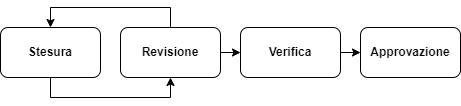
\includegraphics[scale=0.8]{img/ciclo_di_vita.png}
    \caption{Ciclo di vita dei documenti}
\end{figure}
\newpage
\subsubsection{Struttura dei documenti}
Tutti i documenti ufficiali seguono una struttura ben definita cosi da mantenere l'omogeneità. Più precisamente ogni documento è composto da:
\begin{itemize}
    \item \textbf{Frontespizio};
    \item \textbf{Registro delle modifiche};
    \item \textbf{Indice};
    \item \textbf{Contenuto principale}.
\end{itemize}

\subsubsubsection{Frontespizio}
Rappresenta la pagina iniziale del documento ed è strutturato come segue:
\begin{itemize}
    \item \textbf{Logo dell'università}: Logo dell'\textit{Università di Padova} posizionato nella parte centrale alta della pagina, seguito dalla nomenclatura "Università degli  Studi di Padova";
    \item \textbf{Logo del gruppo}: Logo del gruppo, posizionato in centro, a seguito della nomenclatura dell'università;
    \item \textbf{Nome del gruppo e del progetto}: Il nome del gruppo e del capitolato scelto, seguito dal recapito email del gruppo;
    \item \textbf{Nome del documento}: Il titolo del documento, definito in grassetto e posizionato al centro della pagina;
    \item \textbf{Tabella di descrizione}: Tabella contenente le informazioni generali del documento.
\end{itemize}

\subsubsubsection{Registro delle modifiche}
I documenti che sono soggetti a modifiche periodiche sono dotati di un registro che ne memorizza lo storico. Questo è impostato come segue:
\begin{itemize}
    \item \textbf{Versione}: Indica la versione del documento dopo una particolare modifica;
    \item \textbf{Descrizione}: Descrive brevemente la modifica apportata;
    \item \textbf{Data}: Indica la data in cui è stato modificato il documento.
\end{itemize}

\subsubsubsection{Indice}
Per agevolare la lettura, tutti i documenti sono dotati di un indice. Le sezioni sono rappresentate da un numero identificativo seguito dal titolo della sezione. Ogni sottosezione deve riportare il numero della sezione genitore e poi il proprio numero identificativo. I numeri partono dall'uno.

\subsubsubsection{Contenuto principale}
Le varie pagine di contenuto sono costituite da:
\begin{itemize}
    \item \textbf{Intestazione}: In alto a sinistra deve esserci il nome del gruppo \textit{Catch em All}, mentre in altro a destra si trova il numero e nome della sezione in cui ci si trova;
    \item \textbf{Pie di pagina}: In basso sinistra si trova il nome del documento e la sua versione attuale, mentre in basso a destra viene indicato il numero della pagina in cui ci si trova insieme al numero di pagine complessive del documento.
\end{itemize}

\subsubsection{Classificazione dei documenti}
Tutti i documenti prodotti sono divisi in uso interno e uso esterno:
\begin{itemize}
    \item \textbf{Uso interno}: Sono documenti finalizzati a un uso interno al gruppo, questi sono \textit{Norme di progetto} e \textit{Verbali interni};
    \item \textbf{Uso esterno}: Sono documenti di interesse a tutti gli stakeholder, questi sono \textit{Analisi dei requisiti\textsubscript{G}}, \textit{Verbali esterni}, \textit{Piano di progetto}, \textit{Piano di qualifica}, \textit{Glossario}.
\end{itemize}

\subsubsection{Norme tipografiche}

\subsubsubsection{Nome del file}
Di seguito viene descritto il formato dei nomi dei documenti:
\begin{itemize}
\item Iniziano tutti con la lettera minuscola;
\item Se il nome comprende più parole allora ognuna di esse è separata dal simbolo '\_';
\item Deve essere seguito dalla versione in cui si trova.
\end{itemize}
La sigla della versione deve essere così strutturata:
\begin{center}
    \large{\textbf{\_v.X.Y.Z}}
\end{center}
Dove:
\begin{itemize}
\item \textbf{X}: Indicato da un numero che parte da 0, corrisponde al numero di approvazioni del documento da parte del responsabile;
\item \textbf{Y}: Indicato da un numero che parte da 0, corrisponde al numero di verifiche del documento da parte dei verificatori, viene portato a 0 ad ogni incremento di \textbf{X};
\item \textbf{Z}: Indicato da un numero che parte da 0, corrisponde al numero di modifiche del documento da parte del redattore, viene portato a 0 ad ogni incremento di \textbf{X} e \textbf{Y}.
\end{itemize}
Esempio corretto: Norme\_di\_progetto\_v.0.0.1, Norme\_di\_progetto\_v.0.2.1, Norme\_di\_progetto\_v.1.0.0.
Esempi non corretti: Norme\_di\_progetto, NormeDiProgetto.\\
I verbali non seguono questa norma e hanno una nomenclatura diversa, poiché non subiscono variazioni dopo la prima redazione e hanno il seguente formato: 
\begin{center}
	\verb|V<<Tipo di verbale>>_<<Data verbale>>|
\end{center}
Dove:
\begin{itemize}
	\item \verb|V| sta a indicare che si tratta di un verbale;
	\item \verb|Tipo di verbale| indica se è interno (|VI|) o esterno(|VE|);
	\item \verb|Data verbale| indica la data in cui è stato redatto, ed deve essere scritta nel formato YYYYMMDD.
\end{itemize}

\subsubsubsection{Stile di testo}
Di seguito vengono riportati i vari stili del testo e i loro utilizzi:
\begin{itemize}
\item \textbf{Grassetto}: Utilizzato per i termini da descrivere all'interno degli elenchi puntati e per i titoli delle varie sezioni del documento. Può essere utilizzato anche per evidenziare concetti particolarmente rilevanti;
\item \textbf{Corsivo}: Utilizzato per il nome e l'email del gruppo, il nome del progetto, riferimenti ad altri documenti e sigle;
\item \textbf{Link}: Sono collegamenti esterni al documento.
\end{itemize}

\subsubsubsection{Glossario}
Le norme da seguire relative al \textit{Glossario} sono:
\begin{itemize}
    \item Ogni parola presente nel documento \textit{Glossario v 1.0.0} viene contrassegnata con una 'G' a pedice all'interno dei vari documenti dove è utilizzata;
    \item Se un termine compare nella sua stessa definizione all'interno del \textit{Glossario } esso viene contrassegnato.
\end{itemize}

\subsubsubsection{Elenchi puntati e numerati} \label{sec:elenchi_puntati_numerati}
Di seguito vengono descritti come utilizzare elenchi puntati e numerati:
\begin{itemize}
\item La frase introduttiva all'elenco deve terminare con \textbf{':'};
\item Ogni punto dell'elenco inizia con la lettera maiuscola;
\item Alla fine di ogni punto vi è un \textbf{';'};
\item Dopo l'ultima voce vi è un \textbf{'.'}.
\end{itemize}

\subsubsubsection{Sigle}
Di seguito viene elencata una lista di sigle le quali si possono trovare nei documenti e i loro significati:
\begin{itemize}
\item \textbf{Documentazione}:
	\begin{itemize}
	\item \textbf{AdR}: Indica l' \textit{Analisi Dei requisiti\textsubscript{G}};
	\item \textbf{NdP}: Indica le \textit{Norme Di Progetto};
	\item \textbf{PdP}: Indica il \textit{Piano Di Progetto};
	\item \textbf{PdQ}: Indica il \textit{Piano Di Qualifica};
	\item \textbf{Gls}: Indica il \textit{Glossario}.
	\end{itemize}
\item \textbf{Ruoli}:
	\begin{itemize}
	\item \textbf{Re}: Indica il ruolo di \textit{Responsabile di Progetto};
	\item \textbf{Am}: Indica il ruolo di \textit{Amministratore di Progetto};
	\item \textbf{An}: Indica il ruolo di \textit{Analista};
	\item \textbf{Pt}: Indica il ruolo di \textit{Progettista};
	\item \textbf{Pr}: Indica il ruolo di \textit{Programmatore};
	\item \textbf{Ve}: Indica il ruolo di \textit{Verificatore}.
	\end{itemize}
\item \textbf{Revisioni di progetto}:
	\begin{itemize}
		\item \textbf{RTB}: Indica la prima revisione di progetto, e comprende la Requirements and Technology baseline\textsubscript{G};
		\item \textbf{PB}: Indica la seconda revisione, e comprende la Product Baseline;
		\item \textbf{CA}: Indica la terza revisione, e comprende la Customer Acceptance.
	\end{itemize}
\end{itemize}
\subsubsubsection{Formato della data}
Il team ha adottato il seguente formato per le date all'interno dei documenti:
\begin{center}
    \large{\textbf{DD-MM-YYYY}}
\end{center}
Dove \textbf{DD} indica il giorno, \textbf{MM} indica il mese e \textbf{YYYY} indica l'anno.

\subsubsection{Elementi grafici}

\subsubsubsection{Tabelle}
Ogni tabella del documento deve:
\begin{itemize}
\item Essere centrata orizzontalmente;
\item Essere accompagnata da una didascalia che indichi il numero della tabella all'interno del documento. L'unica eccezione è la tabella delle modifiche che non necessita di didascalie.
\end{itemize}

\subsubsubsection{Immagini}
Ogni immagine del documento deve:
\begin{itemize}
\item Essere centrata orizzontalmente;
\item Essere accompagnata da una didascalia che indichi il numero dell'immagine all'interno del documento.
\end{itemize}

\subsubsection{Strumenti}
Di seguito vengono elencati gli strumenti usati per redigere i documenti:
\begin{itemize}
\item \textbf{\LaTeX}: Per la produzione dei documenti, il team ha deciso di usare il linguaggio di markup \textit{\LaTeX};
\item \textbf{Microsoft Word}: Per la stesura delle bozze di alcune parti di documenti;
\item \textbf{Microsoft Excel}: Per la creazione delle tabelle con i preventivi delle ore e costi che verranno poi inserite nel \textit{PdP};
\item \textbf{StarUML}: Per la creazione dei vari UML\textsubscript{G} da inserire all'interno dei documenti;
\item \textbf{LucidChart}: Per discussioni di gruppo sui vari UML\textsubscript{G} creati, dato che lo strumento permette modifiche condivise.
\end{itemize}


\subsection{Gestione della configurazione}

\subsubsection{Scopo}
Lo scopo di questa sezione è descrivere come il team ha deciso di mantenere traccia delle attività e del loro risultato durante il corso del progetto. 

\subsubsection{Sistemi software utilizzati}
La gestione delle versioni dei documenti viene effettuata utilizzato il sistema di controllo di versione Git, attraverso il servizio di GitHub\textsubscript{G}. Per la scrittura dei verbali interni ed esterni si è deciso di utilizzare il servizio Confluence offerto da JIRA\textsubscript{G}.
Al fine di una migliore organizzazione sono stati creati 3 repository per: documentazione, PoC\textsubscript{G} e RTB.
\subsubsection{Strutture dei repository\textsubscript{G}}
Di seguito vengono illustrati i conenuti dei repository:
\begin{itemize}
	\item \textbf{Docs} è il repository\textsubscript{G} contenente documentazione riguardante:
	\begin{itemize}
		\item \textbf{Assegnazione appalto}: Con al suo interno i documenti \textit{lettera\_candidatura.pdf}, 
		\textit{preventivo\_ore\_costi\_rischi.pdf}, 
		\textit{motivazione\_capitolati.pdf};
		\item \textbf{Norme di progetto};
		\item \textbf{Analisi dei requisiti\textsubscript{G}};
		\item \textbf{Piano di progetto};
		\item \textbf{Piano di qualifica};
		\item \textbf{Glossario};
		\item \textbf{Link dei verbali interni ed esterni};
		\item \textbf{Ricerce ed approfondimenti riguardanti nuove tecnologie da adottare}.
	\end{itemize}
	\item \textbf{PoC\textsubscript{G}} è il repository\textsubscript{G} contente il PoC\textsubscript{G} composto da:
	\begin{itemize}
		\item PoC\textsubscript{G} Immagini;
		\item PoC\textsubscript{G} Proof of work\textsubscript{G}.
	\end{itemize}
	\item \textbf{RTB} è il repository\textsubscript{G} contiene tutti i documenti (alla versione \textit{1.0.0}) necessari per RTB.
\end{itemize}
\subsubsection{Struttura delle cartelle su Confluence}
Confluence, un servizio fornito da JIRA\textsubscript{G} è utilizzato dal gruppo per la scrittura e l'organizzazione di:
\begin{itemize}
	\item \textbf{Verbali}: Interni ed esterni;
	\item \textbf{Sprint\textsubscript{G} retrospective}: Contenente le varie analisi retrospettive del gruppo sugli sprint\textsubscript{G} svolti.
\end{itemize}
Tale scelta è stata guidata dalla qualità dei template forniti dallo strumento, i quali facilitano la scrittura e la comprensione di alcuni specifici documenti.

\subsubsection{Gestione delle modifiche}
Per evitare i conflitti tra le modifiche, mantenere in ordine i file e garantire che all'interno del branch\textsubscript{G} principale ci siano solo documenti verificati, il gruppo ha deciso che ogni qual volta sia necessaria una modifica in uno specifico documento deve essere creato un branch\textsubscript{G} per apportarla. La modifica in questione potrà essere integrata nel branch\textsubscript{G} principale soltanto se revisionata con successo dal \textit{Ve}.

\subsubsection{Tipi di file presenti}
Nella repository\textsubscript{G} \textit{Docs} sono presenti esclusivamente file \textit{.tex}, \textit{.txt}, \textit{.png} e \textit{.pdf}. Altri file prodotti durante la stesura dei documenti con estensioni diverse da quelle citate sono escluse attraverso il file \textit{.gitignore}.



\subsection{Assicurazione della qualità}
\subsubsection{Scopo}
Questo processo ha lo scopo di assicurare che tutti i processi e prodotti siano conformi con gli obiettivi e le metriche definiti dal gruppo nel documento \textit{Piano\_di\_qualifica v 1.0.0}. 
Devono essere continuamente osservate la qualità di processo\textsubscript{G} per garantire una buona gestione del progetto e la qualità del prodotto per assicurarsi di lavorare in modo conforme alle richieste del proponente.
\subsubsection{Denominazione obiettivi di qualità}
Ogni obiettivo sarà contrassegnato da un codice univoco così composto:
\begin{center}
	\verb|OQ<<Tipo di obiettivo>><<ID>>|
\end{center}
Dove:
\begin{itemize}
	\item \verb|OQ| sta per obiettivo di qualità;
	\item \verb|<<Tipo di obiettivo>>| identifica se è di processo o prodotto (PC-PD);
	\item \verb|<<ID>>| è un contatore correlato al tipo di obiettivo.
\end{itemize}
\subsubsection{Denominazione metriche di qualità}
Ogni metrica sarà contrassegnata da un codice univoco così composto:
\begin{center}
	\verb|MQ<<Tipo di metrica>><<ID>>|
\end{center}
Dove:
\begin{itemize}
	\item \verb|MQ| sta per metrica di qualità;
	\item \verb|<<Tipo di metrica>>| identifica se è di processo o prodotto (PC-PD);
	\item \verb|<<ID>>| è un contatore correlato al tipo di metrica.
\end{itemize}
\subsubsection{Dettagli metriche di qualità}
\subsubsubsection{Metriche di processo}
Le metriche di qualità a cui ogni processo deve essere conforme sono:
\begin{itemize}
	\item \textbf{SPICE}: Riferito alla metrica per misurare il miglioramento continuo (MQPC01);
	\item \textbf{Costo pianificato di progetto}: Riferito alla metrica per misurare l'efficienza dell'utilizzo delle risorse (MQPC02);
	\item \textbf{Costo pianificato di progetto svolto}: Riferito alla metrica per misurare l'efficienza dell'utilizzo delle risorse (MQPC03);
	\item \textbf{Costo reale di progetto svolto}: Riferito alla metrica per misurare l'efficienza dell'utilizzo delle risorse (MQPC04);
	\item \textbf{Variazioni nella pianificazione}: Riferito alla metrica per misurare le variazioni dalla pianificazione (MQPC05);
	\item \textbf{Variazioni nei costi}: Riferito alla metrica per misurare le variazioni dalla pianificazione (MQPC06).
\end{itemize}
\paragraph{SPICE}\mbox{}\\
Questa metrica è di riferimento ai processi ed è stata scelta dal gruppo per verificare il grado di \textit{capability}\textsubscript{G} che ogni processo deve raggiungere. Lo standard definisce vari livelli di \textit{capability}\textsubscript{G}:
\begin{itemize}
	\item \textbf{Livello 0 - Incomplete process}: Il processo non è implementato oppure è incapace di raggiungere i suoi obiettivi;
	\item \textbf{Livello 1 - Performed process}: Il processo è attivo e può essere completato ma non è sottoposto a controlli;
	\item \textbf{Livello 2 - Managed process}: Il processo processo è attivo e pianificato, e può completare i suoi obbiettivi attraverso vari controlli;
	\item \textbf{Livello 3 - Established process}: Il processo è definito da degli standard;
	\item \textbf{Livello 4 - Predictable process}: Il processo è attivo secondo standard e viene controllato in modo dettagliato per renderlo in futuro prevedibile e ripetibile;
	\item \textbf{Livello 5 - Optimizing process}: Il processo è completamente definito e tracciato, e viene analizzato e migliorato in maniera continua.
\end{itemize}
Per misurare la \textit{capability}\textsubscript{G} si utilizzano i vari attributi di un processo:
\begin{itemize}
	\item Process performance;
	\item Performance management;
	\item Work product management;
	\item Process definition;
	\item Process deployment;
	\item Process measurement;
	\item Process control;
	\item Process innovation;
	\item Process optimization.
\end{itemize}
Ogni attributo di processo viene valutato su una scala di valutazione NPLF\textsubscript{G}.\\ Il gruppo si impegna a raggiungere un grado di \textit{capability}\textsubscript{G} minimo di 2 per ogni processo.
\paragraph{Costo pianificato di progetto}\mbox{}\\
Questa metrica è di riferimento ai processi ed è stata scelta dal gruppo per indicare il costo totale di progetto pianificato alla data corrente. Il valore si può osservare nella sezione \textit{Preventivo} del \textbf{Piano di progetto}. Questo valore deve essere $\geq$ 0 e minore del budget totale disponibile.
\paragraph{Costo pianificato di progetto svolto}\mbox{}\\
Questa metrica è di riferimento ai processi ed è stata scelta dal gruppo per indicare il valore effettivo del prodotto ottenuto fino alla data corrente.
\paragraph{Costo reale di progetto svolto}\mbox{}\\
Questa metrica è di riferimento ai processi ed è stata scelta dal gruppo per indicare il costo reale impiegato per svolgere il progetto fino alla data corrente. Il valore si può osservare nella sezione \textit{Consuntivo} del \textbf{Piano di progetto}. Questo valore deve essere un intorno\textsubscript{G} del BCWS con un errore non superiore al 20\%.
\paragraph{Variazioni nella pianificazione}\mbox{}\\
Questa metrica è di riferimento ai processi ed è stata scelta dal gruppo per misurare in che percentuale ci sono state variazioni rispetto alla pianificazione preventivata. Questa metrica si calcola come segue:
\begin{align*}
	\centering
	\textbf{VP} = \frac{100 * (BCWP - BCWS)}{BCWS}
\end{align*}
Dove:
\begin{itemize}
	\item \textbf{VP} sta per \textit{Variazione pianificazione};
	\item \textbf{BCWP} sta per \textit{Budgeted Cost of Work Performed};
	\item \textbf{BCWS} sta per \textit{Budgeted Cost of Work Scheduled}.
\end{itemize}
\paragraph{Variazioni nei costi}\mbox{}\\
Questa metrica è di riferimento ai processi ed è stata scelta dal gruppo per misurare in che percentuale ci sono state variazioni tra i costi di sviluppo pianificati e quelli reali. Questa metrica si calcola come segue:
\begin{align*}
	\centering
	\textbf{VC} = \frac{100 * (BCWS - ACWP)}{BCWS}
\end{align*}
Dove:
\begin{itemize}
	\item \textbf{VC} sta per \textit{Variazione costi};
	\item \textbf{ACWP} sta per \textit{Actual Cost of Work Performed};
	\item \textbf{BCWS} sta per \textit{Budgeted Cost of Work Scheduled}.
\end{itemize}
\subsubsubsection{Metriche di prodotto}
Le metriche di qualità a cui ogni prodotto deve essere conforme sono divisi in due categorie:
\begin{itemize}
	\item \textbf{Metriche per la qualità della documentazione};
	\item \textbf{Metriche per la qualità del software}.
\end{itemize}
\subsubsubsection{Metriche di qualità della documentazione}
Le metriche di qualità a cui solo la documentazione deve essere conforme sono:
\begin{itemize}
	\item \textbf{Indice di Gulpease}: Che fa riferimento alla metrica \textit{MQPD01};
	\item \textbf{Correttezza ortografica}: Che fa riferimento alla metrica \textit{MQPD02}.
\end{itemize}
\paragraph{Indice di Gulpease}\mbox{}\\
L'indice di Gulpease è una metrica di riferimento ai prodotti di documentazione che il gruppo ha scelto di utilizzare per verificare la leggibilità della documentazione prodotta. L'indice è tarato sulla lingua italiana e si calcola in questo modo:
\begin{align*}
	\centering
	\textbf{IG} = 89 + \frac{300 * Nfrasi - 10 * Nlettere}{Nparole}
\end{align*}
Il gruppo ha scelto come valore minimo di accettabilità 40. Questo viene indicato come limite dato che un valore minore implica una difficoltà di lettura anche per chi ha conferito un diploma di scuola superiore.
\paragraph{Correttezza ortografica}\mbox{}\\
Questa metrica è di riferimento ai prodotti di documentazione ed è utilizzata dal gruppo per assicurare la correttezza ortografica di ogni parola presente nei documenti. Non devono esserci errori grammaticali per far sì che un documento sia accettato.
\subsubsubsection{Metriche di qualità del software}
Le metriche di qualità a cui solo il software deve essere conforme sono:
\begin{itemize}
	\item \textbf{Copertura funzionale}: Che fa riferimento alla metrica \textit{MQPD03};
	\item \textbf{Tempo di risposta dei servizi all'utente}: Che fa riferimento alla metrica \textit{MQPD04};
	\item \textbf{Copertura dei test}: Che fa riferimento alla metrica \textit{MQPD05};
	\item \textbf{Robustezza agli errori}: Che fa riferimento alla metrica \textit{MQPD06};
	\item \textbf{Completezza di descrizione}: Che fa riferimento alla metrica \textit{MQPD07};
	\item \textbf{Completezza della guida utente}: Che fa riferimento alla metrica \textit{MQPD08};
	\item \textbf{Interfaccia utente auto-esplicativa}: Che fa riferimento alla metrica \textit{MQPD09};
	\item \textbf{Procedure di autenticazione}: Che fa riferimento alla metrica \textit{MQPD10};
	\item \textbf{Accoppiamento\textsubscript{G} di componenti}: Che fa riferimento alla metrica \textit{MQPD11};
	\item \textbf{Adeguatezza della complessità ciclomatica}\textsubscript{G}: Che fa riferimento alla metrica \textit{MQPD12};
	\item \textbf{Completezza della funzione di test}: Che fa riferimento alla metrica \textit{MQPD13};
	\item \textbf{Browser supportati}: Che fa riferimento alla metrica \textit{MQPD14}.
\end{itemize}
\paragraph{Copertura funzionale}\mbox{}\\
Questa metrica è di riferimento ai prodotti software ed è utilizzata dal gruppo per verificare che tutti i requisiti obbligatori del progetto siano stati integrati nel prodotto finale. Questa metrica è calcolata attraverso il rapporto tra il numero di requisiti soddisfatti e quello di requisiti obbligatori totali:
\begin{align*}
	\centering
	\textbf{CF} = \frac{RqSoddisfatti}{RqTotali}
\end{align*}
Dove \textbf{CF} sta per \textit{Copertura funzionale}.
\paragraph{Tempo di risposta dei servizi all'utente}\mbox{}\\
Questa metrica è di riferimento ai prodotti software ed è utilizzata dal gruppo per assicurare che i tempi di risposta del prodotto siano accettabili. Un tempo di risposta adeguato in un sistema CAPTCHA\textsubscript{G} è molto importante e per questo è un obiettivo fondamentale. Il valore accettabile verrà analizzato in una fase più avanzata di progetto.
\paragraph{Copertura dei test}\mbox{}\\
Questa metrica è di riferimento ai prodotti software ed è utilizzata dal gruppo per verificare che i test svolti sul prodotto finale coprano tutti i requisiti e casi d’uso identificati. Questa metrica è calcolata attraverso il rapporto tra il numero di requisiti e casi d'uso testati e quello di requisiti e casi d'uso totali da testare:
\begin{align*}
	\centering
	\textbf{CdT} = \frac{RqUCTestati}{RqUCTotali}
\end{align*}
Dove \textbf{CdT} sta per \textit{Copertura dei test}.
\paragraph{Robustezza agli errori}\mbox{}\\
Questa metrica è di riferimento ai prodotti software ed è utilizzata dal gruppo per verificare quale parte di tutti gli errori critici, ovvero quelli che possono determinare blocchi del sistema, è stata messa sotto controllo. Questa metrica è calcolata attraverso il rapporto tra il numero di errori critici gestiti e il numero totale di errori critici da gestire in totale:
\begin{align*}
	\centering
	\textbf{RaE} = \frac{ErrCritGestiti}{ErrCritTotali}
\end{align*}
Dove \textbf{RaE} sta per \textit{Robustezza agli errori}.
\newpage
\paragraph{Completezza di descrizione}\mbox\\
Questa metrica è di riferimento ai prodotti software ed è utilizzata dal gruppo per verificare la percentuale degli scenari d’uso che è descritta nella documentazione rispetto al totale. Questo per poter garantire informazioni complete agli utilizzatori del prodotto. Questa metrica è calcolata attraverso il rapporto tra il numero di scenari descritti e il numero di scenari effettivamente presenti nel dominio\textsubscript{G}:
\begin{align*}
	\centering
	\textbf{CdD} = \frac{ScenariDescritti}{ScenariPresenti}
\end{align*}
Dove \textbf{CdD} sta per \textit{Completezza di descrizione}.
\paragraph{Completezza della guida utente}\mbox{}\\
Questa metrica è di riferimento ai prodotti software ed è utilizzata dal gruppo per verificare la percentuale delle funzioni utilizzabili dall'utente che hanno una descrizione completa nei vari manuali. Questa metrica è calcolata attraverso il rapporto tra il numero di funzionalità descritte e il numero di funzionalità totali:
\begin{align*}
	\centering
	\textbf{CdGU} = \frac{FunzDescritte}{FunzTotali}
\end{align*}
Dove \textbf{CdGU} sta per \textit{Completezza della guida utente}.
\paragraph{Interfaccia utente auto-esplicativa}\mbox{}\\
Questa metrica è di riferimento ai prodotti software ed è utilizzata dal gruppo per verificare la percentuale degli elementi di informazione che sono presentati all’utente inesperto in modo che possa completare un’attività senza un addestramento preliminare o assistenza esterna. Questa metrica è calcolata attraverso il rapporto tra il numero di informazioni fornite all'utente rispetto a quelle di cui avrebbe bisogno per completare ogni piccolo passo:
\begin{align*}
	\centering
	\textbf{IUAE} = \frac{InfoFornite}{InfoRichieste}
\end{align*}
Dove \textbf{IUAE} sta per \textit{Interfaccia utente auto-esplicativa}.
\paragraph{Procedure di autenticazione}\mbox{}\\
Questa metrica è di riferimento ai prodotti software ed è utilizzata dal gruppo per verificare il grado di efficacia del sistema CAPTCHA\textsubscript{G} implementato per l'autenticazione di un utente. Il gruppo definisce un grado di accettabilità per la percentuale di accessi indesiderati non bloccati:
\begin{center}
	\textbf{AINB} $\le$ 25\%
\end{center}
Dove \textbf{AINB} sta per \textit{Accessi indesiderati non bloccati}.
\paragraph{Accoppiamento\textsubscript{G} di componenti}\mbox{}\\
Questa metrica è di riferimento ai prodotti software ed è utilizzata dal gruppo per controllare quanti componenti del sistema sono strettamente  indipendenti e quanti sono esenti da impatti conseguenti a cambiamenti negli altri componenti.
In futuro verrà definito un valore per misurarla al meglio. 
\newpage
\paragraph{Adeguatezza della complessità ciclomatica}\textsubscript{G}\mbox{}\\
Questa metrica è di riferimento ai prodotti software ed è utilizzata dal gruppo per verificare quanti moduli software hanno una complessità ciclomatica\textsubscript{G} accettabile. Per verificarla il gruppo deciderà una soglia di accettabilità per i vari linguaggi di programmazione e per il tipo di modulo o di funzione utilizzati durante il progetto.\\
Nelle metriche software la complessità ciclomatica\textsubscript{G} è usata per valutare la complessità di un algoritmo ed è basata sulla struttura del grafo che rappresenta l’algoritmo da misurare. Per calcolarla si fa uso di questa formula:
\begin{align*}
	\centering
	\textbf{v(G)} = L - N + 2 * P
\end{align*}
Dove:
\begin{itemize}
	\item \textbf{v(G)}: Numero ciclomatico relativo al grafo G;
	\item \textbf{L}: Numero di archi nel grafo;
	\item \textbf{N}: Numero di nodi del grafo;
	\item \textbf{P}: Numero dei componenti del grafo disconnessi.
\end{itemize}
\paragraph{Completezza della funzione di test}\mbox{}\\
Questa metrica è di riferimento ai prodotti software ed è utilizzata dal gruppo per verificare la percentuale di completezza delle funzioni di test implementate. Questa metrica è calcolata attraverso il rapporto tra il numero di test implementati e il numero di test totali da fare:
\begin{align*}
	\centering
	\textbf{CdFT} = \frac{TestImpl}{TestTot}
\end{align*}
Dove \textbf{CdFT} sta per \textit{Completezza della funzione di test}.
\paragraph{Browser supportati}\mbox{}\\
Questa metrica è di riferimento ai prodotti software ed è utilizzata dal gruppo per verificare il numero di browser che supportano il prodotto sviluppato. Il gruppo definirà un grado di accettabilità per la percentuale di browser che deve supportare il prodotto.
\begin{center}
	\textbf{BRS} $\geq$ 75\%
\end{center}
Dove \textbf{BRS} sta per \textit{Browser supportati}.

\subsection{Verifica\textsubscript{G}}
\subsubsection{Scopo}
Questo processo ha lo scopo di confermare che ciascuna attività svolta soddisfi i requisiti\textsubscript{G} e gli obiettivi specificati, attraverso le metriche scelte dal gruppo e descritte in dettaglio nel documento \textit{Piano\_di\_qualifica v 1.0.0} e che non abbia introdotto errori.
Il processo di \textit{verifica\textsubscript{G}} deve essere integrato nei processi di \textit{Fornitura}, \textit{Sviluppo} e \textit{Manutenzione}.
\newline
\newline
Il processo di verifica\textsubscript{G} è suddiviso in due fasi:
\begin{itemize}
	\item \textbf{Analisi statica}, la quale non richiede l'esecuzione dell'oggetto di verifica\textsubscript{G};
	\item \textbf{Analisi dinamica}, la quale richiede l'esecuzione dell'oggetto di verifica\textsubscript{G}.
\end{itemize}

\subsubsection{Analisi statica}
L’analisi statica si occupa di analizzare la documentazione e il codice e accerta la conformità alle regole introdotte, l'assenza di errori, la completezza dei requisiti\textsubscript{G} desiderati. Inoltre poiché non richiede l’esecuzione dell’oggetto di verifica\textsubscript{G}, si può applicare ad ogni prodotto di processo.\\
Si utilizzano due metodi per svolgere analisi statica:
\begin{itemize}
	\item \textbf{Walkthrough};
	\item \textbf{Inspection}.
\end{itemize}
Queste sono effettuate tramite studio dell’oggetto di verifica\textsubscript{G} e lettura umana o automatizzata.
\subsubsubsection{Walkthrough}
\paragraph {Scopo}\mbox{}\\
I verificatori, insieme agli sviluppatori quando necessario, che utilizzano questo metodo devono rilevare la presenza di errori attraverso una lettura critica ad ampio spettro del prodotto da analizzare. Questo metodo è molto oneroso dal punto di vista delle risorse utilizzate, e perciò si cercherà di utilizzare solo fino al momento in cui non sarà disponibile una checklist.
\paragraph {Fasi:}\:
\begin{enumerate}
	\item Pianificazione, svolta da autori e verificatori;
	\item Lettura, svolta dai verificatori;
	\item Discussione, svolta da autori e verificatori;
	\item Correzione degli errori, svolta dagli autori.
\end{enumerate}
\paragraph {}\mbox{}\\
\subsubsubsection{Inspection}
\paragraph {Scopo}\mbox{}\\
I verificatori che utilizzano questo metodo devono rilevare la presenza di errori eseguendo una lettura mirata dell’oggetto di verifica\textsubscript{G} attraverso l'utilizzo di una checklist. Si cerca quindi di immaginare in precedenza quali saranno le criticità dell'oggetto da analizzare e di elencarli.
\paragraph {Fasi:}\:
\begin{enumerate}
	\item Pianificazione;
	\item Definizione di una checklist;
	\item Lettura;
	\item Correzione degli errori, svolta dagli autori.
\end{enumerate}
Per garantire e mantenere la qualità dei documenti elevata durante il loro intero sviluppo (quindi lungo
l’intero arco di vita del progetto) il gruppo si è impegnato nello sviluppo di 2 programmi di analisi statica:
uno riguardante i documenti e l'altro per le parole del glossario.\\
Etrambi gli script\textsubscript{G} sono eseguibili da qualunque ambiente di sviluppo e sono stati sviluppati in python\textsubscript{G}.\\
La loro semplice e breve esecuzione permette un controllo frequente.\\
Sono stati, inoltre, integrati e resi obbligatori nel repository pubblico attraverso le branch protection rules\textsubscript{G} di GitHub\textsubscript{G}.
\paragraph{File correctness script\textsubscript{G}}\mbox{}\\
Questo script\textsubscript{G} permette di controllare la correttezza dei file di testo (ad esempio i file .tex) e delle cartelle.\\
Il programma permette di verificare determinati elementi:
\begin{itemize}
	\item All'interno del file;
	\item Nomi dei file;
	\item Nomi delle cartelle;
	\item Strutture delle cartelle.
\end{itemize}
\noindent Queste verifiche sono per la maggior parte delegate ad un modulo chiamato "specific\_rules" il quale contiene tutte le verifiche da fare tramite espresssioni regolari (regex). \\
La struttura di questo programma prevede una checklist di macro controlli da effettuare (contenuta nel file principale "file\_correctness.py") i quali a loro volta contengono una serie di controlli più specifici (contenuti nel modulo "checks" il quale si avvale del modulo "specifics\_rules"). \\
I documenti analizzati sono:
\begin{itemize}
	\item Analisi dei requisiti\textsubscript{G};
	\item Norme di progetto;
	\item Piano di progetto;
	\item Piano di qualifica;
	\item Glossario.
\end{itemize}
\noindent Le verifiche effettuate dallo script\textsubscript{G} in generale sono:
\begin{itemize}
	\item Presenza delle cartelle contententi i file sopra citati;
	\item Correttezza nome cartella;
	\item Struttura delle cartelle:
		\begin{itemize}
			\item Presenza di una sola cartella "src":
				\begin{itemize}
					\item Presenza di una cartella "sections" (contenente i file LaTeX che compongono il documento);
					\item Eventuale presenza della cartella "img" contenente immagini necessarie al documento.
				\end{itemize}
			\item Presenza di un unico file "pdf" il quale identifica il documento.
		\end{itemize}
\end{itemize}
In particolare:
\begin{itemize}
	\item Ogni documento deve avere 
	\begin{lstlisting}
		'font size': r'.*\\documentclass\[10pt\]\{article\}.*',
		'packages file': r'.*\\input\{sections/packages\}.*',
		'style file': r'.*\\input\{sections/style\}.*',
		'title page': r'.*\\input\{sections/title_page\}.*',
		'page roman numbering': r'.*\\pagenumbering\{roman\}.*',
		'table of contents': r'.*\\tableofcontents.*',
		\end{lstlisting}
		\item Controllo della presenza di almeno un file LaTeX nella cartella "sections" e di nessun altro tipo di file;
		\item Controllo della presenza dei file necessari nella cartella "sections", precedentemente inclusi nel file LaTeX in "src";
	Ovvero:
	\begin{lstlisting}
	necessary_sections_files = [
		'style.tex',
		'packages.tex',
		'title_page.tex',
		'modifiche.tex',
		]
	\end{lstlisting}
	\item Controllo della presenza di determinati parametri nel file title\_page.tex, tra cui il titolo che coincida con il nome della cartella in cui si trova il file;
	\item Controllo della presenza di determinati parametri nel file style.tex, tra cui la correttezza del nome del file;
	\item Controllo della presenza di determinati parametri nel file modifiche.tex, tra cui il giusto ordine e l'assenza di ripetizioni nel numero delle versioni;
	\item Controllo della presenza dell'ultima versione nei file title\_page.tex e in style.tex;
	\item Controllo del nome e della correttezza della versione del file pdf;
	\item Controllo del rispetto della norma per le gli elenchi puntati e numerati (\ref{sec:elenchi_puntati_numerati}).
\end{itemize}

\paragraph{Glossario script\textsubscript{G}}\mbox{}\\
Lo script\textsubscript{G} per le parole del glossario verifica queste ultime siano identificate correttamente all'interno dei documenti.\\
In caso contrario il programma segnala l'errore (o warning in casi particolari) e consente di correggerlo.\\


\subsubsection{Analisi dinamica}
L'analisi dinamica si occupa di eseguire dei test sugli oggetti di verifica\textsubscript{G} che devono essere eseguiti. Questo permetterà al gruppo di accertarsi dell'assenza di errori noti.
I test dovranno essere:
\begin{itemize}
	\item \textbf{Ripetibili}, ovvero che garantiscano la correttezza dell'oggetto di verifica\textsubscript{G} e quindi la rimozione di eventuali errori;
	\item \textbf{Automatizzati}, ovvero svolti in maniera automatica da precisi strumenti selezionati.
\end{itemize}
Inoltre verranno eseguiti diversi tipi di test:
\begin{itemize}
	\item \textbf{Test di unità};
	\item \textbf{Test di integrazione};
	\item \textbf{Test di sistema};
	\item \textbf{Test di regressione};
	\item \textbf{Test di accettazione e collaudo}.
\end{itemize}
\subsubsection{Denominazione test di verifica\textsubscript{G}}
Ogni test sarà contrassegnato da un codice univoco così composto:
\begin{center}
	\verb|TV<<Tipo di test>><<ID>>|
\end{center}
Dove:
\begin{itemize}
	\item \verb|TV| sta per test di verifica\textsubscript{G};
	\item \verb|<<Tipo di test>>| identifica il tipo di test che si vuole fare, questi possono essere:
	\begin{itemize}
		\item UN, di unità;
		\item IN, di integrazione;
		\item ST, di sistema;
		\item RG, di regressione;
		\item AC, di accettazione e collaudo.
	\end{itemize}
	\item \verb|<<ID>>| è un contatore correlato al tipo di test.
\end{itemize}
Informazioni più dettagliate sui vari test, strumenti e metriche utilizzate per la verifica\textsubscript{G} si possono trovare nel documento \textit{Piano\_di\_qualifica v 1.0.0}.

\subsection{Validazione\textsubscript{G} e collaudo}
\subsubsection{Scopo}
Lo scopo di questo processo è quello di confermare che tutti i requisiti\textsubscript{G} siano rispettati all'interno del prodotto finale, dopo aver svolto tutti i test di verifica\textsubscript{G}. Questi due processi sono strettamente legati fra loro e una buona verifica\textsubscript{G} durante il corso del progetto permette di superare anche il processo di validazione\textsubscript{G}.
Questo processo permette anche di confermare che il prodotto finale sia conforme alle richieste del proponente.

\subsection{Usabilità}
\subsubsection{Scopo}
Questo processo ha lo scopo di assicurare che siano prese in considerazione, ed  opportunamente indirizzate, le considerazioni espresse dalle parti interessate, gli stakeholders, relativamente alla facilità d'uso del prodotto finale da parte degli utenti cui è rivolto, al supporto che ne riceverà, alla formazione, all'incremento della produttività, alla qualità del lavoro, all'accettazione del prodotto stesso. 



